\FloatBarrier
\section{Aufgabe 2}
\label{sec:Aufgabe2}
%\lstinputlisting[language=Python, firstline=15, lastline=21]{plots/plot.py}
\paragraph{a} 
A beschreibt Messprozess der die verschmierung in Nachbar-Bin mit Wahrscheinlichkeit $\epsilon$ beschreibt, 
z.B. Klassifizierung von Ereignissen in mehere Klassen. 
Ergebnis der geschriebenen Methode für $n= 4$ und $ \epsilon = 0.23$ :
\begin{equation}
\begin{pmatrix}
0.77& 0.23& 0.  & 0.  \\
0.23& 0.54& 0.23& 0.  \\
0.  & 0.23& 0.54& 0.23\\
0.  & 0.  & 0.23& 0.77
\end{pmatrix}
\label{eq:ma}
\end{equation}

\paragraph{b}
gmess er gibt sich zu: 
\begin{equation}
g_{mess} = [254,474,616,758,826,770,759,729,691,610,563,487,459,407,341,318,247,223,194,181]
\end{equation}
\paragraph{c}
Mit Transformation von $A = UDU^{-1}$ und $U$ transformationsmatrix und $D$ Diagonalmatrix folgt
\begin{gather}
g = A\cdot f = UDU^{-1} \cdot f \\
\iff \underbrace{U^{-1} g}_{=c} = D \underbrace{U^{-1} \cdot f}_{=b} \\
\iff c = D\cdot b  \; .
\label{eq:cdb}
\end{gather}
Vorteil: Die Einträge $b_j$ und $c_j$ können unabhängig transfomiert werden, da $D$ Diagonalmatrix. 

\paragraph{d}
Aus den Gleichungen aus \textbf{b} kann man dann $f$ und $b$ leicht durch Matrixmultiplikation 
brechnen. Die Kovarianz $V[b]$ von $b = D^{-1} U^{-1} g_{mess}$ lässt sich berechnen mit 
$B = D^{-1} U^{-1} $ und $V[b] = BV[g_{mess}]B^T$. Die Koeffizienten normiert auf ihre Standardabweichung 
sind in der Abbildung \ref{fig:bjplot} dargestellt. Alle Werte die um 1 liegen haben eine große Abweichung 
in der Größenordnung des Wertes. 
Folglich sind dies die Werte, 
die verstärkt von statistischen Fluktuationen betroffen sind und somit kommt es dann zu Oszillationen.
 
\begin{figure}
  \centering
  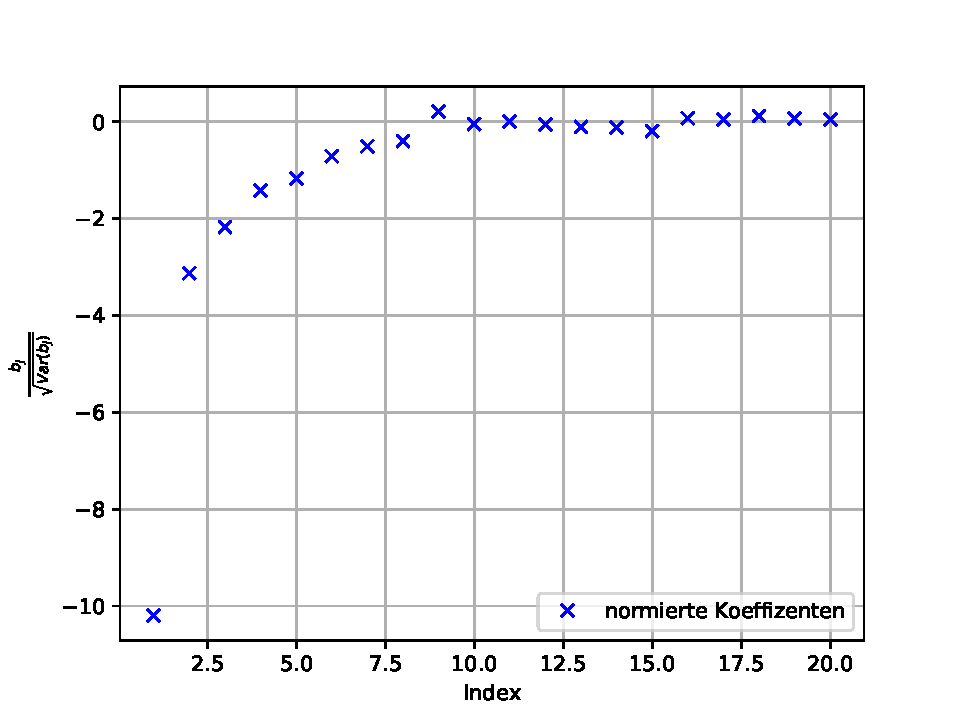
\includegraphics[height = 10cm]{plots/bjggIndexplot.pdf}
  \caption{Einträge von b normiert auf ihre Standardabweichung gegen ihren Index aufgetragen.}
  \label{fig:bjplot}
\end{figure}

\paragraph{e}
Die Werte mit Regularisierung sind nähr an der wahren Verteilung dran und zeigen auch kleine Fehler. 
Siehe dazu Abbildung \ref{fig:rplot}. 
\begin{figure}
  \centering
  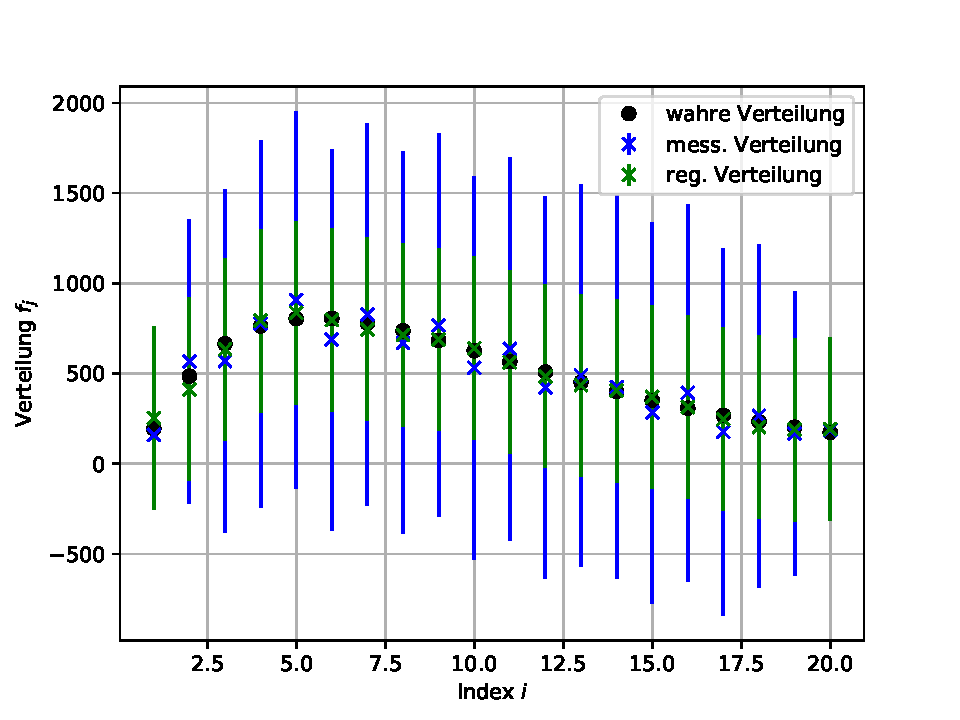
\includegraphics[height = 10cm]{plots/regplot.pdf}
  \caption{Wahre, gemessene und die regularisierte Verteilung gegen den Index Aufgetragen.}
  \label{fig:rplot}
\end{figure}
\FloatBarrier

